\chapter{Project Design}
In this chapter, we have detailed our project requirement, methods and design structure. Finally, give a summary of this chapter. 

\section{System Design}
\label{Sys_des}
\subsection{Context Diagram}
Our tool mainly consist of three stack-holders. They are students, researchers and doctors. Users will give the gene expression data to the server via a web UI (User Interface) and then the server will do the classification and analysis job and return the result summary back to the user.
\begin{figure}[H]
    \centering
    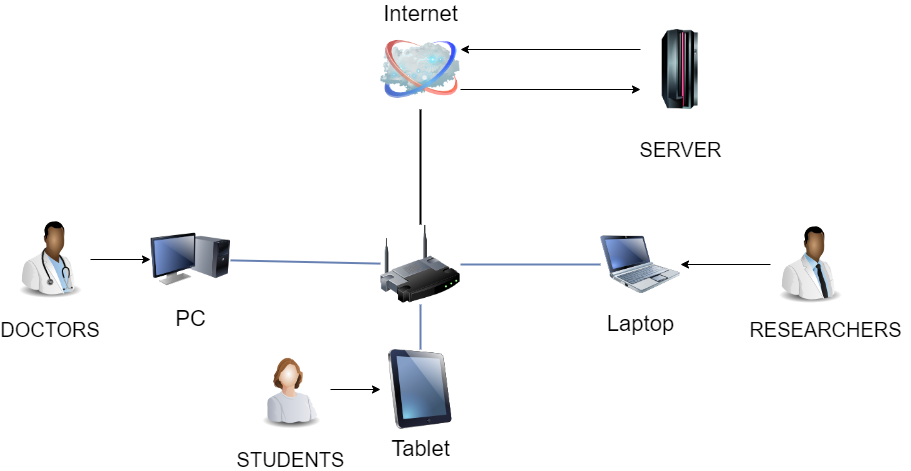
\includegraphics[width=0.70\textwidth]{context.png}
    \caption{Context diagram of our tool \index{context diagram} }
    \label{fig:contextfig}
\end{figure}
\subsection{Data Flow Diagram}
Here is our data flow diagram \ref{fig:DFDfig} which shows how the data will flow through the system from taking input from user to show the report to the user. 
\begin{figure}[H]
    \centering
    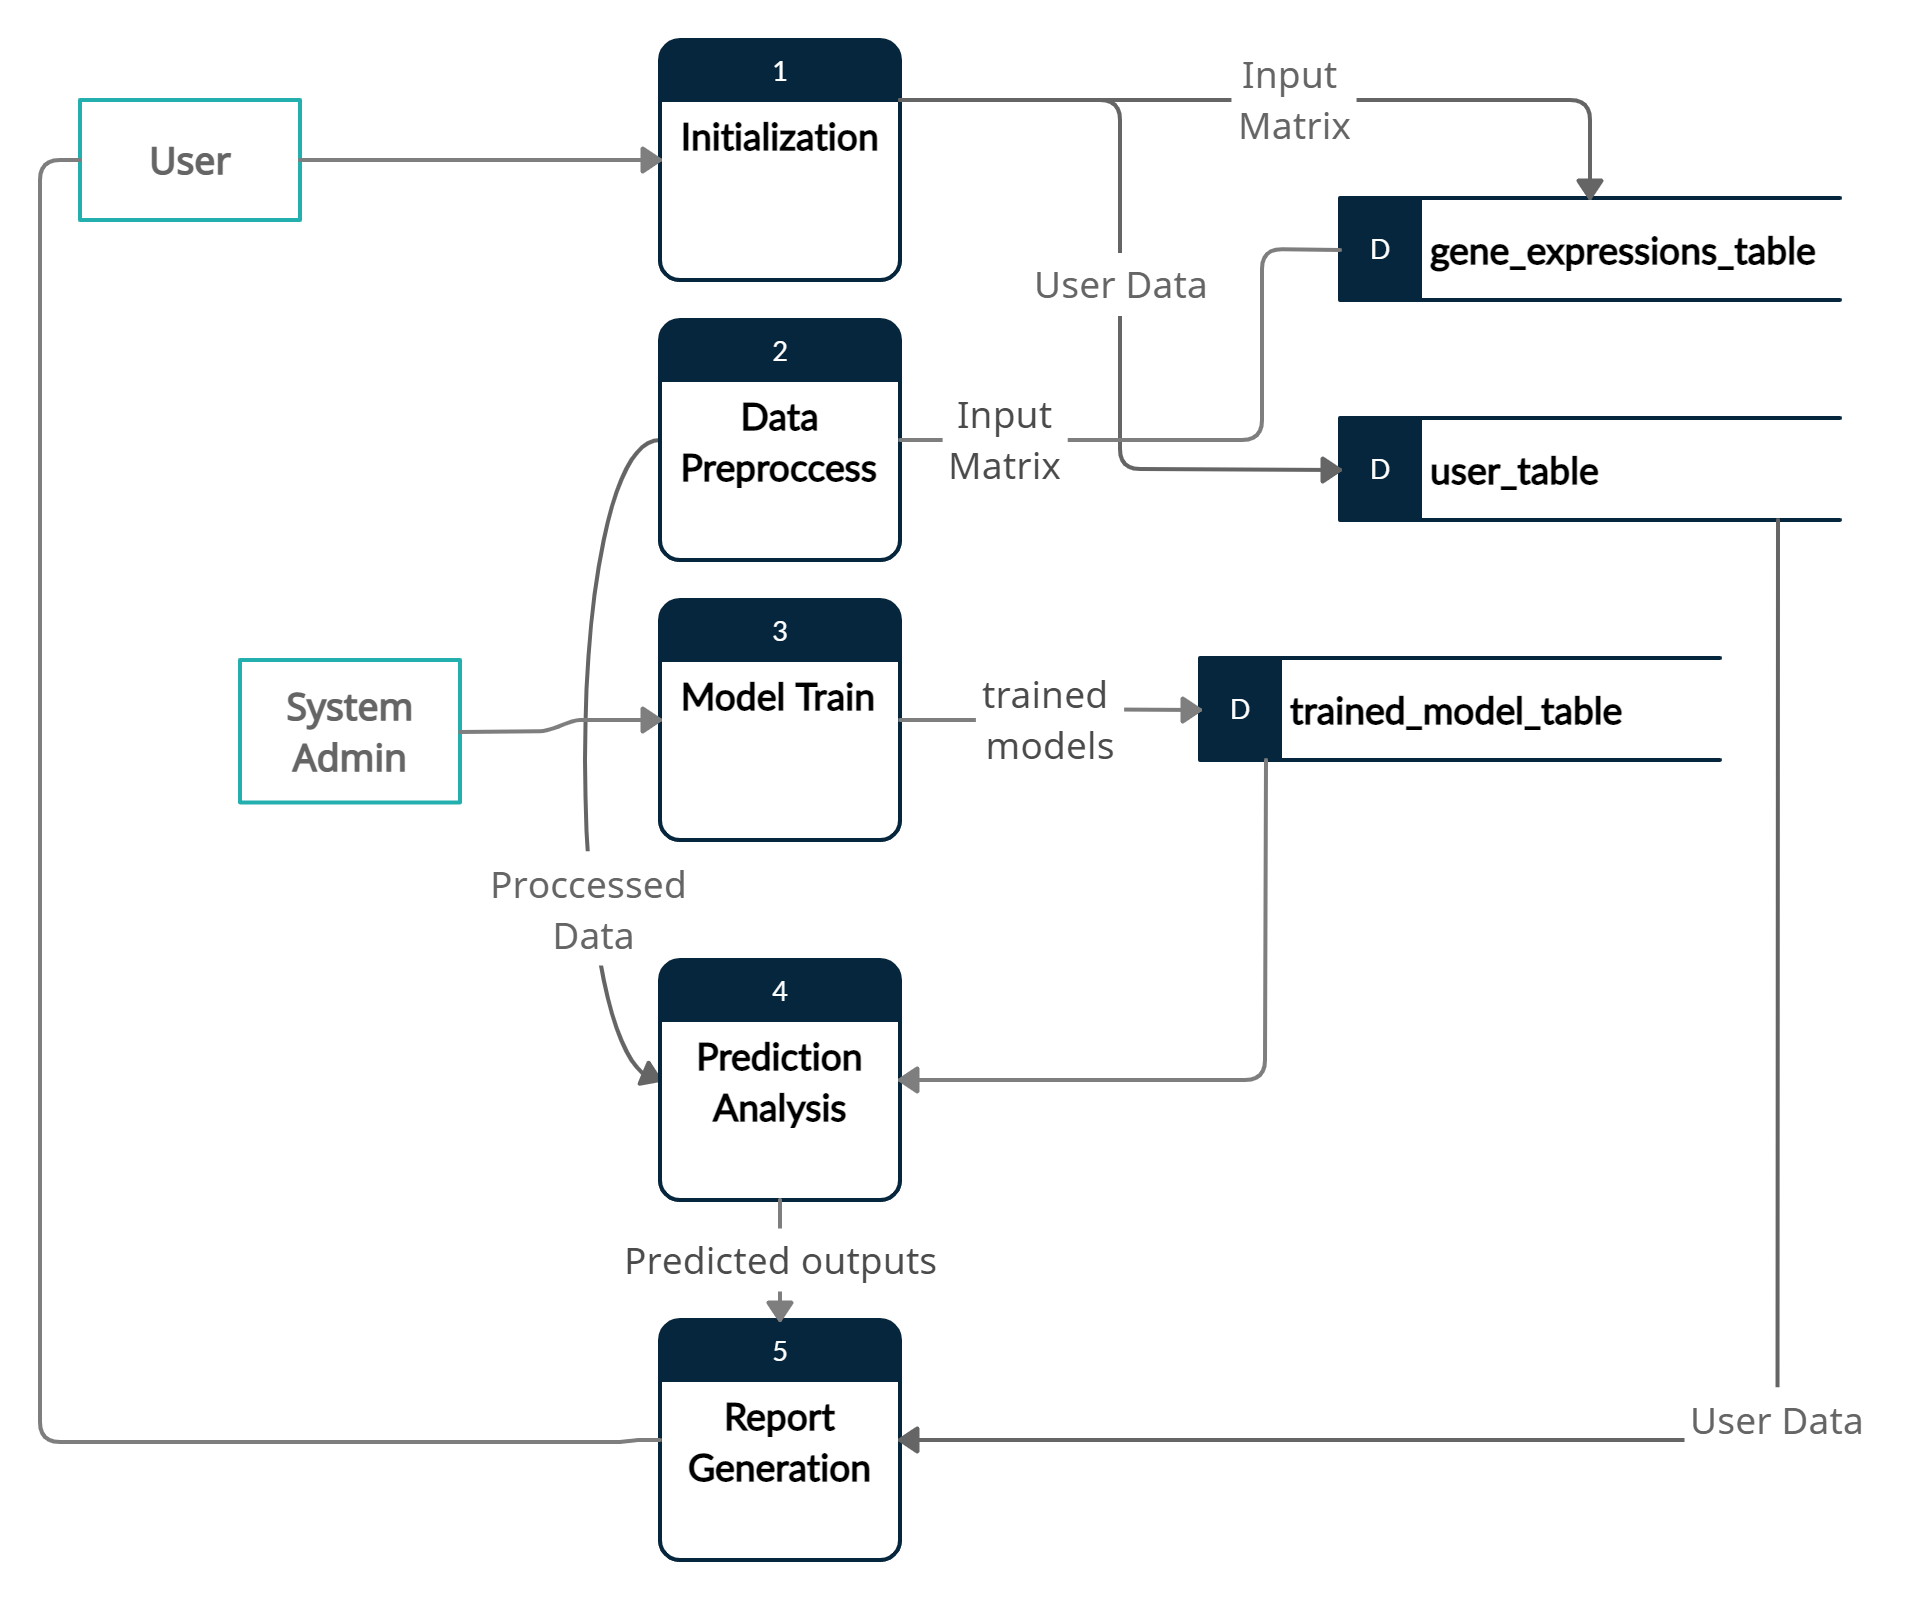
\includegraphics[width=0.70\textwidth]{DFD.png}
    \caption{Data flow diagram of our tool \index{Data Flow Diagram} }
    \label{fig:DFDfig}
\end{figure}
\section{Methodology and Design}
\label{Meth_des}
\subsection{Data Collection}
We have collected 22 types of cancer data from TCGA (The Cancer Genome Atlas) using TCGA2STAT. TCGA2STAT is a R package available in cran archive \cite{tcga}. At first we had to know the name code of cancer ex. (BRCA, CHOL, READ. Using this code we downloaded TCGA \index{The Cancer Genome Atlas} data directly from the TCGA archive website \cite{GDC}. We also collected data from GEO ( Gene Expression Omnibus ) using the accession code directly from the NCBI website \cite{GEO}. 
\subsection{Pre-processing}
At first, we had to transform the collected data into cell in rows and genes in columns formation. Dropped indices and columns with unnecessary values. In some cases, we had to distinct different classes by the given meta data and some other cases, we had to add target values with the data-set. Then for TCGA data, we standardized the data using StandardScaler from sklearn. 
\subsection{Gene Selection}
For gene selection, at first we did F-ANOVA on TCGA cancer data and selected n - best genes from each cancer data. Then merge all the best genes. We prepared multiple dataset with various m genes to do binary classification and pan cancer classification. 
\begin{figure}[H]
    \centering
    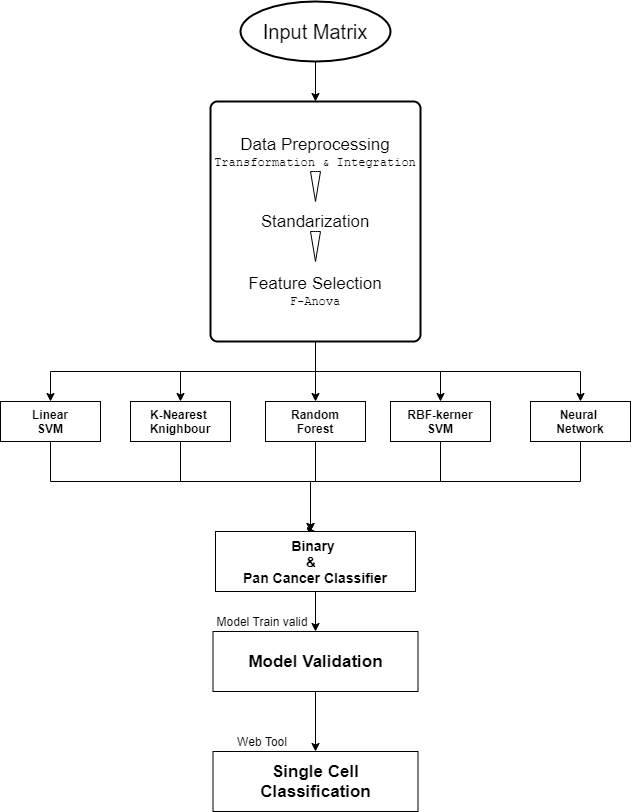
\includegraphics[width=0.70\textwidth]{Workflow.png}
    \caption{Workflow of our Tool \index{Pan Tool} }
    \label{fig:workflowfig}
\end{figure}
In the above figure \ref{fig:workflowfig} we have shown a visual flow of our total work flow how we prepare and process data then which methods are used to prepare the classifier and finally how the classification is done
\section{Summary}
